\input{header_xe.tex}
\def \labnum {1}
\def \labsubj {Теория автоматов}
\def \labauthor {Чебыкин И. Б.}
\def \labgroup {P3301}
\def \labinsp {Ожиганов А. А.}
\def \labname {Вариант: 12}
\isnametrue

\usepackage{listings,longtable,amsmath,amsfonts,graphicx,tikz,tabularx,pgf}
\usepackage{caption}
\usetikzlibrary{arrows,automata}

\captionsetup{labelsep=period}
\pagestyle{fancy}
\begin{document}
\input{title.tex}

\section{Описание работы}
Цель -- практическое освоение методов взаимного преобразования автоматных
моделей Милли и Мура. Проверка абстрактных автоматов Мили и Мура на эквивалентность.

Исходный абстрактный автомат задан графическим способом. При переходе
от автомата Мура к Мили и наоборот учесть, что их входные и выходные алфавиты
должны совпадать.
\section{Порядок выполнения задания}
\begin{enumerate}
\item В соответствии с выбранным номером варианта осуществить преобразование автомата Мили в автомат Мура (Мура в Мили).
\item Сформировать входное слово необходимой длины. Длина входного слова должна быть минимальна, но достаточна для осуществления всех имеющихся в графах автоматов переходов.
\item Используя сформированное входное слово, осуществить проверку исходного и полученного в результате преобразования автоматов на эквивалентность. В качестве исходного состояния выбрать состояние а1.
\end{enumerate}
\newpage
\section{Выполнение}
    \subsection{Граф автомата Мили}
	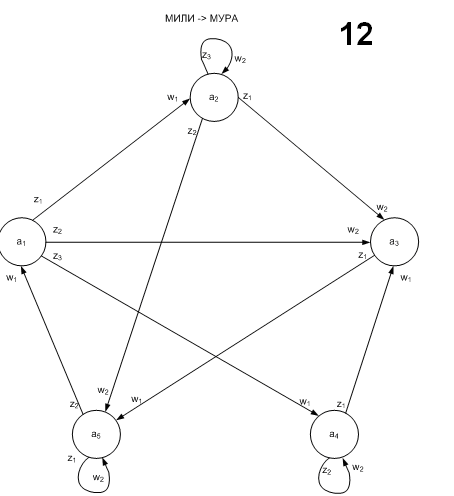
\includegraphics{img/mealy.png}
    \subsection{Преобразованный автомат Мура}
	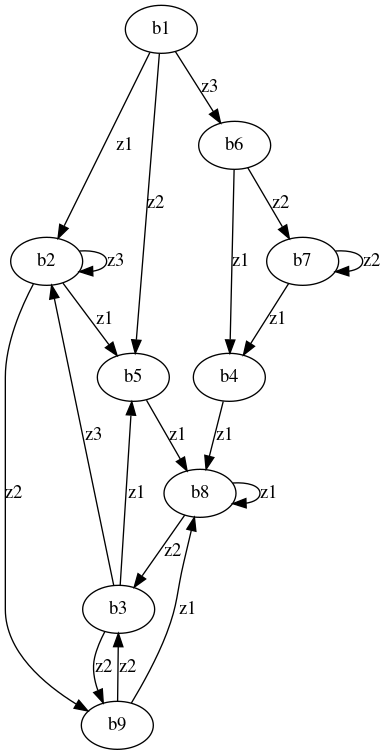
\includegraphics[width=200bp]{img/moore.png}
\newpage
\section{Этапы преобразования автоматов}
        $S_b = (A_b, Z_b, W_b, {\delta}_b, {\lambda}_b, a_{1b})$
        где \\
        $A_b$ -- множество состояний автомата Мили; \\
        $Z_b$ -- входной алфавит; \\
        $W_b$ -- выходной алфавит; \\
        ${\delta}_b$ -- функция переходов автомата; \\
        ${\lambda}_b$ -- функция выходов автомата; \\
        $a_{1b}$ -- начальное состояние.

        В эквивалентном автомате Мура $Z_b = Z_a$, $W_b = W_a$.

        Построим таблицу автомата Мили:

        \begin{table}[!h]
        \centering
            \begin{tabular} {|c|c|c|c|c|c|}
                \hline
                $\delta$ & $a_1$ & $a_2$ & $a_3$ & $a_4$ & $a_5$ \\ \hline
                $z_1$  & $a_2$ & $a_3$ & $a_5$ & $a_3$ & $a_5$ \\ \hline
                $z_2$  & $a_3$ & $a_5$ &       & $a_4$ & $a_1$ \\ \hline
                $z_3$  & $a_4$ & $a_2$ &       &       &       \\ \hline
            \end{tabular}
            \caption{Таблица переходов автомата Мили}
        \end{table}
        \begin{table}[!h]
        \centering
            \begin{tabular} {|c|c|c|c|c|c|}
                \hline
                $\lambda$ & $a_1$ & $a_2$ & $a_3$ & $a_4$ & $a_5$ \\ \hline
                $z_1$  & $w_1$ & $w_2$ & $w_1$ & $w_1$ & $w_2$ \\ \hline
                $z_2$  & $w_2$ & $w_2$ &       & $w_2$ & $w_1$ \\ \hline
                $z_3$  & $w_1$ & $w_2$ &       &       &       \\ \hline
            \end{tabular}
            \caption{Таблица выходов автомата Мили}
        \end{table}

        По таблице определим пары $(a_s, w_g)$, определяющие эквивалентные состояния в автомате Мура. \\
        $A_1 = \{ (a_1, w_1) \} = \{ b_1 \}$ \\
        $A_2 = \{ (a_2, w_1), (a_2, w_2) \} = \{ b_2, b_3 \}$ \\
        $A_3 = \{ (a_3, w_1), (a_3, w_2) \} = \{ b_4, b_5 \}$ \\
        $A_4 = \{ (a_4, w_1), (a_4, w_2) \} = \{ b_6, b_7 \}$ \\
        $A_5 = \{ (a_5, w_1), (a_5, w_2) \} = \{ b_8, b_9 \}$


        Составим таблицу переходов для автомата Мура. Для этого смотрим на состояние в исходной паре,
        ищем следующее множество состояний для автомата Мура из функции $\delta(a_s, z_f)$ и определяем
        состояние для автомата Мура из функции $\lambda(a_s, z_f)$ для автомата Мили.

        \begin{table}[!h]
        \centering
            \begin{tabular} {|c|c|c|c|c|c|c|c|c|c|} \hline $\delta$  & $b_1$ & $b_2$ & $b_3$ & $b_4$ & $b_5$ & $b_6$ & $b_7$ & $b_8$ & $b_9$ \\ \hline
                $\lambda$ & $w_1$ & $w_1$ & $w_2$ & $w_1$ & $w_2$ & $w_1$ & $w_2$ & $w_1$ & $w_2$ \\ \hline
                $z_1$     & $b_2$ & $b_5$ & $b_5$ & $b_8$ & $b_8$ & $b_4$ & $b_4$ & $b_8$ & $b_8$ \\ \hline
                $z_2$     & $b_5$ & $b_9$ & $b_9$ & -     & -     & $b_7$ & $b_7$ & $b_3$ & $b_3$ \\ \hline
                $z_3$     & $b_6$ & $b_2$ & $b_2$ & -     & -     & -     & -     & -     & -     \\ \hline
            \end{tabular}
            \caption{Таблица выходов автомата Мура}
        \end{table}

\section{Реакции автоматов на входное слово}
        \subsection{Входное слово минимальной длины}
		Находим слово минимальной длины методом перебора: \\
            $z_1 z_3 z_1 z_1 z_1 z_2 z_1 z_2 z_2 z_2 z_1 z_2 z_3 z_2 z_1$
        \subsection*{Реакция автоматов}
        \begin{table}[!h]
        \centering
            \begin{tabular}{|c|c|}
                \hline
                Состояние   & Слово \\ \hline
                $(a_1,z_1)$ & $w_1$ \\ \hline
                $(a_2,z_3)$ & $w_2$ \\ \hline
                $(a_2,z_1)$ & $w_2$ \\ \hline
                $(a_3,z_1)$ & $w_1$ \\ \hline
                $(a_5,z_1)$ & $w_2$ \\ \hline
                $(a_5,z_2)$ & $w_1$ \\ \hline
                $(a_1,z_1)$ & $w_1$ \\ \hline
                $(a_2,z_2)$ & $w_2$ \\ \hline
                $(a_5,z_2)$ & $w_1$ \\ \hline
                $(a_1,z_2)$ & $w_2$ \\ \hline
                $(a_3,z_1)$ & $w_1$ \\ \hline
                $(a_5,z_2)$ & $w_1$ \\ \hline
                $(a_1,z_3)$ & $w_1$ \\ \hline
                $(a_4,z_2)$ & $w_2$ \\ \hline
                $(a_4,z_1)$ & $w_1$ \\ \hline
            \end{tabular}
            \caption{Реакция автомата Мили}
        \end{table}
        \begin{table}[!h]
        \centering
            \begin{tabular}{|c|c|}
                \hline
                Состояние   & Слово \\ \hline
                $(b_1,z_1)$ & -     \\ \hline
                $(b_2,z_3)$ & $w_1$ \\ \hline
                $(b_3,z_1)$ & $w_2$ \\ \hline
                $(b_5,z_1)$ & $w_2$ \\ \hline
                $(b_8,z_1)$ & $w_1$ \\ \hline
                $(b_8,z_2)$ & $w_2$ \\ \hline
                $(b_1,z_1)$ & $w_1$ \\ \hline
                $(b_2,z_2)$ & $w_1$ \\ \hline
                $(b_9,z_2)$ & $w_2$ \\ \hline
                $(b_1,z_2)$ & $w_1$ \\ \hline
                $(b_5,z_1)$ & $w_2$ \\ \hline
                $(b_8,z_2)$ & $w_1$ \\ \hline
                $(b_1,z_3)$ & $w_1$ \\ \hline
                $(b_6,z_2)$ & $w_1$ \\ \hline
                $(b_7,z_1)$ & $w_2$ \\ \hline
                $(b_4)$     & $w_1$ \\ \hline
            \end{tabular}
            \caption{Реакция автомата Мура}
        \end{table}


        Реакция автомата Мили: $w_1w_2 w_2 w_1 w_1 w_1 w_1 w_2 w_1 w_2 w_1 w_1 w_1 w_2 w_1$. \\
        Реакция автомата Мура: $w_1w_2 w_2 w_1 w_1 w_1 w_1 w_2 w_1 w_2 w_1 w_1 w_1 w_2 w_1$. \\
		Реакции двух автоматов совпадают, значит можно сказать, что автоматы
		эквивалентны.


\section{Вывод}
В ходе выполнения данной лабораторной работы были изучены автоматы Мили и Мура
и способы их преобразования.
В данной работе был использован табличный способ преобразования автоматов.
Исходя из результата преобразования можно заметить, что в эквивалентном автомате
Мура больше состояний, следовательно, в данном случае лучше подходит автомат Мили.
\end{document}
